
\begin{center}
	\Huge
	Eulers metode
\end{center}
\section*{Eulers metode}
\stepcounter{section}

Vi har kun stiftet bekendtskab med differentialligninger, vi kan finde en eksplicit løsning til - altså differentialligninger, der har en eller anden form for funktionsforskrift som løsning. Det viser sig, at dette ikke nødvendigvis er tilfældet, og derfor kan vi få brug for at approksimere løsninger til differentialligninger ud fra et begyndelsespunkt. Et sådan problem kaldes ofte for et \textit{begyndelsesværdiproblem}, og disse har vi en række forskellige måder at approksimere. Én disse kaldes for \textit{Eulers metode}.

Lad os prøve at motivere metoden. Vi forestiller os at have en differentialligning med begyndelsesbetingelse givet ved
\begin{align*}
	y' = d(x,y), \quad y(x_0) = y_0,
\end{align*}
hvor $d$ er en funktion, der afhænger af $x$ og $y$. Dette kunne eksempelvis være
\begin{align*}
	y' = d(x,y) = x\cdot y - y^2, \quad y(2) = 5.
\end{align*}
Vi kender ikke forskrift for løsningen $f$ til differentialligningen, men vi kender $y'$ i $(x_0,y_0)$ samt punktet $(x_0,y_0)$. 
Vi kan derfor tegne en tangent i $(x_0,y_0)$, og bevæge os et kort stykke $h$ hen langs tangenten. Hvis $h$ er lille, må forskellen mellem tangentens $y$-værdi og funktionsværdien for $f$ være relativt lille. Vores bud på en ny $x$- og $y$-værdi er derfor 
\begin{align}
\begin{split}
	\label{eq:euler1}
	x_1 &= x_0 + h,\\
	y_1 &= y_0 + h\cdot d(x_0,y_0),
\end{split}
\end{align}
da $d(x_0,y_0)$ er tangentens hældning i $(x_0,y_0)$ og $h$ er det stykke, vi bevæger os langs $x$-aksen. Vi kan se dette illustreret på Figur \ref{fig:eulertangent}.
\begin{figure}[H]
	\centering
	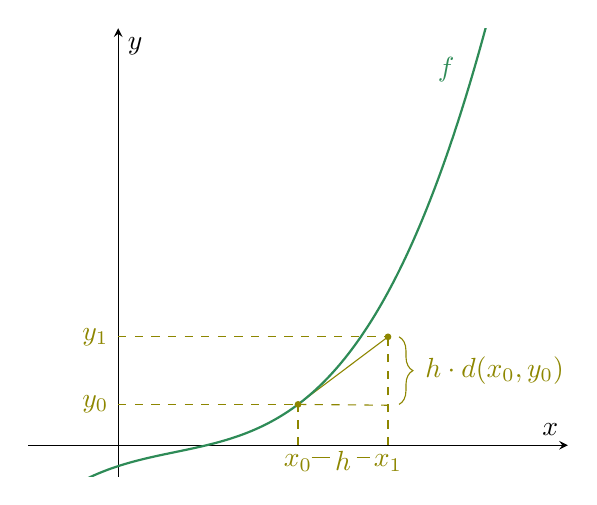
\begin{tikzpicture}
	\begin{axis}[
		axis lines = center, 
		xmin = -1, xmax = 5,
		ymin = -1.5, ymax = 20,
		xlabel = $x$, ylabel = $y$, 
		ticks = none, 
	]
		%Dashes
		\draw[color = olive, dashed] (axis cs: 2,0) -- (axis cs: 2,1.96) node[pos = 0, anchor = north] {$x_0$};
		\draw[color = olive, dashed] (axis cs: 0, 1.96) --
		(axis cs: 2,1.96) node[pos = 0, anchor = east] {$y_0$};
		\draw[color = olive, dashed] (axis cs: 3,0) -- (axis cs: 3, 5.2) node[pos = 0, anchor = north] {$x_1$};
		\draw[color = olive, dashed] (axis cs: 0, 5.2) --
		(axis cs: 3,5.2) node[pos = 0, anchor = east] {$y_1$};
		\draw[color = olive, dashed] (axis cs: 2, 1.96) --
		(axis cs: 3,1.92); 
		\filldraw[color = olive] (axis cs: 3, 5.2) circle (1pt);
		%tangent
		\addplot[color = olive, domain = 2:3] {3.24*x - 4.52};
		%Function
		\addplot[color = SeaGreen, thick, samples = 300,
		domain = -1:5] {0.42*x^3-0.8*x^2+1.4*x - 1};
		%pynt
		\filldraw[color = olive] (axis cs: 2, 1.96) circle (1pt);
		\draw[color = olive] (axis cs: 2.15,-0.6 ) -- (axis cs: 2.35,-0.6);
		\node[color = olive, anchor = north] at (axis cs: 2.5,0.2) {$h$};
		\draw[color = olive] (axis cs: 2.65,-0.6 ) -- (axis cs: 2.80,-0.6);
		\draw[decorate, decoration={brace, amplitude=5pt, mirror, raise = 4pt}, color = olive] 
  		(axis cs:3,1.96) -- (axis cs:3,5.2)
		node[pos = 0.5, anchor = west, xshift = 10pt] {$h\cdot d(x_0,y_0)$};
		\node[color = SeaGreen, anchor = east, xshift = -5pt] at (axis cs: 4, 18,68) {$f$};
	\end{axis}
	\end{tikzpicture}
	\caption{Et enkelt skridt i Eulers metode, der viser, hvordan vi finder $(x_1,y_1)$ som approksimation til den ukendte funktion $f$.}
	\label{fig:eulertangent}
\end{figure}
Vi kan se, at vi i vores approksimation kommer til at ramme lidt under den rigtige løsning. Dette er et centralt problem i Eulers metode, men hvis $h$ vælges lille nok, kan man komme vilkårligt tæt på den rigtige løsning.

Idéen i Eulers metode er at blive ved med at finde nye punkter $(x,y)$ ved at sætte det nuværende fundne punkt ind i ligningerne \eqref{eq:euler1}.

\begin{defn}[Eulers metode]
	Eulers metode for begyndelsesværdiproblemet
	\begin{align*}
		y' = d(x,y), \quad y(x_0) = y_0,
	\end{align*} 
	defineres som proceduren
	\begin{align*}
		x_{n+1} &= x_n + h,\\
		y_{n+1} &= y_n + h\cdot d(x_n,y_n).
	\end{align*}
\end{defn}
På Figur \ref{fig:euler} kan vi se Eulers metode illustreret med forskellige skridtlængder $h$. 
\begin{figure}[H]
	\centering
	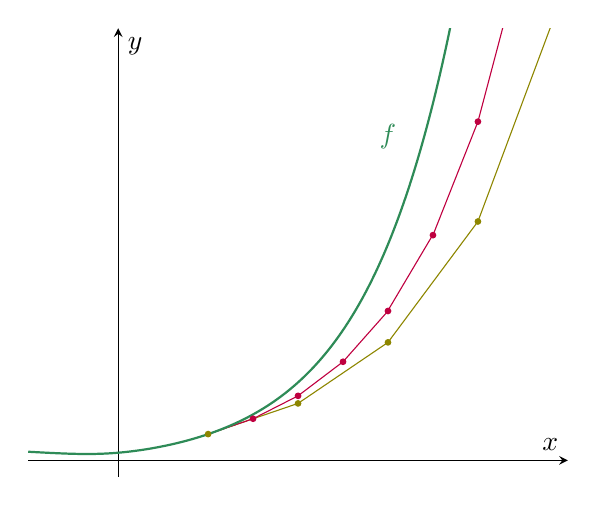
\begin{tikzpicture}
	\begin{axis}[
		axis lines = center, 
		xmin = -1, xmax = 5,
		ymin = -1.5, ymax = 40,
		xlabel = $x$, ylabel = $y$, 
		ticks = none, 
	]
		
		%tangents1
		\addplot[color = olive, domain = 1:2] {2.84*x - 0.41};
		\addplot[color = olive, domain = 2:3] {5.65*x - 6.03};
		\addplot[color = olive, domain = 3:4] {11.19*x - 22.65};
		\addplot[color = olive, domain = 4:5] {22.29*x - 67.05};
		%tangents2
		\addplot[color = purple, domain = 1:1.5] {2.84*x - 0.41};
		\addplot[color = purple, domain = 1.5:2] {4.24*x - 2.510};
		\addplot[color = purple, domain = 2:2.5] {6.31*x - 6.65};
		\addplot[color = purple, domain = 2.5:3] {9.4*x - 14.375};
		\addplot[color = purple, domain = 3:3.5] {14.04*x - 28.245};
		\addplot[color = purple, domain = 3.5:4] {21.01*x - 52.69};
		\addplot[color = purple, domain = 4:4.5] {31.48*x - 94.57};
		\addplot[color = purple, domain = 4.5:5] {47.19*x - 165.265};
		%Function
		\addplot[color = SeaGreen, thick, samples = 300,
		domain = -1:5] {sqrt(-2 + 4*exp(2*x) - 4*x)/2};
		%pynt
		\node[color = SeaGreen] at (axis cs: 3, 30) {$f$};
		%cirkler oliven
		\filldraw[color = olive] (axis cs: 1, 2.43) circle (1pt);
		\filldraw[color = olive] (axis cs: 2, 5.27) circle (1pt);
		\filldraw[color = olive] (axis cs: 3, 10.92) circle (1pt);
		\filldraw[color = olive] (axis cs: 4, 22.11) circle (1pt);
		%cirkler purple
		\filldraw[color = purple] (axis cs: 1.5, 3.85) circle (1pt);
		\filldraw[color = purple] (axis cs: 2, 5.97) circle (1pt);
		\filldraw[color = purple] (axis cs: 2.5, 9.125) circle (1pt);
		\filldraw[color = purple] (axis cs: 3, 13.825) circle (1pt);
		\filldraw[color = purple] (axis cs: 3.5, 20.845) circle (1pt);
		\filldraw[color = purple] (axis cs: 4, 31.35) circle (1pt);
		\filldraw[color = purple] (axis cs: 4.5, 47.09) circle (1pt);
	\end{axis}
	\end{tikzpicture}
	\caption{Eulers metode med to forskellige skridtlængder $h$.}
	\label{fig:euler}
\end{figure}
På Figur \ref{fig:euler} kan vi se, hvordan Eulers metode kommer længere og længere væk fra den korrekte kurve, men også hvordan en mindre skridtlængde $h$ gør, at vi ikke bevæger os så langt fra den korrekte, men ubekendte kurve $f$. 
\begin{exa}
	Vi betragter begyndelsesværdiproblem 
	\begin{align*}
		y' =  \frac{x}{y} + y, \quad y(0) = 2, 
	\end{align*}
	og vi ønsker at anvende Eulers metode med en skridtlængde $h = 1$.
	Den første iteration giver
	\begin{align*}
		x_1 &= x_0 + h \\
		&= 0 + 1 = 1\\
		y_1 &= y_0 + h \cdot d(x_0,y_0) \\
		&= 2 + 1\cdot \left(\frac{0}{2} + 2\right) = 4.
	\end{align*}
	Vi finder nu $x_2$ og $y_2$.
	\begin{align*}
		x_2 &= 1 + 1 = 2 \\
		y_2 &= 4 + 1\cdot \left(\frac{1}{4} + 4 \right) = 8,\! 25. \\
	\end{align*}
	Som det var tilfældet med Newtons metode er dette arbejde for en computer, og vi lader derfor Excel fortsætte arbejdet.
	\begin{table}[H]
		\centering
		\rowcolors{1}{SeaGreen!60}{SeaGreen!30}
		\begin{tabular}{cc}
			$x$ & $y$ \\
			0 & 1 \\
			1 & 4 \\
			2 & $8,\!25$ \\
			3 & $16,\!74$ \\
			4 & $33,\!66$ \\
			5 & $67,\!45$ \\
			6 & $134,\!97$ \\
			7 & $269,\!98$ \\
		\end{tabular}	
		\begin{tabular}{cc}
			$x$ & $y$ \\
			0 &	2 \\
			$1$	 & $4,\!58$ \\
			$2$ &	$10,\!58$ \\
			$3$ &	$24,\!03$ \\
			$4$ &	$54,\!22$\\
			$5$ & 	$122,\!07$ \\	
			$6$	 & $274,\!70$ \\
			$7$ &	$618,\!10$ \\
		\end{tabular}	
		\begin{tabular}{cc}
			$x$ & $y$ \\
			0 &	2 \\
			1 &	$5,\!02$\\
			2	& $12,\!53$  \\
			$3$ &	$30,\!79$\\
			4 &	$75,\!29$\\
			5 &	$183,\!89$\\
			6 &	$448,\!98$\\
			7 &	$1096,\!15$\\
		\end{tabular}	
		\begin{tabular}{cc}
			$x$ & $y$ \\
			0 & 2 \\
			1 & $5,\!29$ \\
			2 & $13,\!87$ \\
			3 & $35,\!78$ \\
			4 & $91,\!90$ \\
			5 & $235,\!85$ \\
			6 & $605,\!18$ \\
			7 & $1552,\!76$ \\
		\end{tabular}	
		\begin{tabular}{cc}
			$x$ & $f(x)$ \\
			0 & 2 \\
			1 & $5,\!63$ \\
			2 & $15,\!59$ \\
			3 & $42,\!56$ \\
			4 & $115,\!80$ \\
			5 & $314,\!82$ \\
			6 & $855,\!80$ \\
			7 & $2326,\!31$ \\
		\end{tabular}	
		\caption{Eulers metode med en skridtlængde på hhv. 1, $\frac{1}{2}$, $\frac{1}{4}$ og $\frac{1}{8}$ og den sande løsning $f$. }
		\label{tab:euler}
	\end{table}
	Vi kan på Tabel \ref{tab:euler} se, at vi særligt med skridtlængde $1$, men også for de andre skridtlængder ender med at komme meget langt væk fra den sande løsning $f$. Eulers metode kræver meget små $h$ for at give gode approksimationer. Derfor anvendes i praksis ofte andre metoder til at approksimere begyndelsesværdiproblemer. 
\end{exa}
\subsection*{Opgave 1}
\begin{enumerate}[label=\roman*)]
	\item Anvend Eulers metode med tre iterationer på følgende begyndelsesværdiproblem med en skridtlængde $h = 1$. 
	\begin{align*}
		y' = x + y, \quad y(0) = 1
	\end{align*}
	\item Anvend Eulers metode med tre iterationer på følgende begyndelsesværdiproblem med en skridtlængde $h = \frac{1}{2}$. 
	\begin{align*}
		y' = 4x + 2y, \quad y(2) = 4
	\end{align*}
	\item Anvend Eulers metode med tre iterationer på følgende begyndelsesværdiproblem med en skridtlængde $h = \frac{1}{2}$. 
	\begin{align*}
		y' = 2x^2y, \quad y(1) = 1
	\end{align*}
\end{enumerate}

\subsection*{Opgave 2}
En differentialligning er givet ved
\begin{align*}
	y' = ax - y
\end{align*}
og det gælder, at $y(1) = 2$. 
\begin{enumerate}[label=\roman*)]
	\item Bestem tallet $a$, hvis det oplyses, at Eulers metode giver $x_1 = 2$ og $y_1 = 4$ med en skridtlængde på $h = 1$.  
\end{enumerate}
\subsection*{Opgave 3}
Et begyndelsesværdiprobleme er givet ved
\begin{align*}
	y' = ax^2 - by, \quad y(0) = 2
\end{align*}
\begin{enumerate}[label=\roman*)]
	\item Bestem tallene $a$ og $b$, hvis det oplyses, at Eulers metode giver $x_1 = 1$, $x_2 = 2$, $y_1 = 8$ og $y_2 = 31$ med en skridtlængde på $h = 1$. 
\end{enumerate}

\subsection*{Opgave 4 (Excel)}
Vi betragter begyndelsesværdiproblemet 
\begin{align*}
	\frac{dy}{dx} = x\sqrt{y}, \quad y(1) = 1.
\end{align*}
Lav Eulers metode i Excel, og udfyld følgende tabel, hvor de korrekte funktionsværdier er udfyldt
\begin{center}
	\rowcolors{1}{SeaGreen!60}{SeaGreen!30}
	\begin{tabular}{cccccc}
		$x$ & $y$ $(h = 1)$ & $y$ $(h = 0,\!5)$ & $y$ $(h = 0,\!1)$ & $y$ $(h = 0,\!01)$ & $f(x)$\\
		$1$ & & & & & $1$\\
		$2$& & & & & $3,\!06$\\
		$3$& & & & & $9$\\
		$4$& & & & & $22,\!56$\\
		$5$& & & & & $49$\\
		$6$& & & & & $95,\!06$\\
		$7$& & & & & $169$\\
	\end{tabular}
\end{center}
Tegn også graferne i Excel i samme koordinatsystem. Ser vi det, vi forventer?